\documentclass{beamer}

\usepackage[spanish,activeacute,es-tabla]{babel}
\usepackage[utf8]{inputenc} % mac utf8
%\usepackage{beamerthemesplit}


\usepackage{graphicx}
\DeclareGraphicsExtensions{.png,.pdf,.jpg}


\usefonttheme{professionalfonts} % fuentes de LaTeX 
\usetheme{Boadilla}	% tema escogido en este ejemplo 


\setbeamertemplate{caption}[numbered]

\newtheorem{Teorema}{Teorema} 
\newtheorem{Ejemplo}{Ejemplo} 
\newtheorem{Definicion}{Definici\’on} 
\newtheorem{Corolario}{Corolario} 
\newtheorem{Prueba}{Prueba}

\newtheorem{teorema} [Teorema] {Teorema}
\newtheorem{ejemplo} [Ejemplo] {Ejemplo}
\newtheorem{definicion} [Definicion]{Definición} 
\newtheorem{ejercicio} [Corolario]{Ejercicio} 
\newtheorem{lema} [theorem] {Lema}

\setbeamertemplate{theorems}[numbered] 





\title[]{Tema 2. Códigos sin prefijos}
\author[José A Montenegro (jmmontes@uma.es)]{José A. Montenegro}
\institute{Dpto. Lenguajes y Ciencias de la Computación\\
ETSI Informática. Universidad de Málaga\\
jmmontes@uma.es
%\href{https://twitter.com//monteDocencia}{
%
\includegraphics[height=0.03\textheight]{twitter.jpg}}
}
\date{\today}

%###########################################################################
% FootLine
%###########################################################################

\setbeamertemplate{footline} {%
\leavevmode%
  \hbox{\begin{beamercolorbox}[wd=.5\paperwidth,ht=2.5ex,dp=1.125ex,leftskip=.3cm plus1fill,rightskip=.3cm]{author in head/foot}%
    \usebeamerfont{author in head/foot}\insertshortauthor 
  \end{beamercolorbox}%
  
  \begin{beamercolorbox}[wd=.5\paperwidth,ht=2.5ex,dp=1.125ex,leftskip=.3cm,rightskip=.3cm plus1fil]{title in head/foot}%
    Teoría de la Información y Codificación \hfill    \insertpagenumber /\insertdocumentendpage
  \end{beamercolorbox}}%
  \vskip0pt%
}%

%###########################################################################
% Document
%###########################################################################

\begin{document}

%\setbeamertemplate{headline}[title slide]
%\setbeamertemplate{footline}[title slide]


%###########################################################################
% Tíitulo
%###########################################################################
\begin{frame}

\includegraphics[height=0.15\textheight]{logoUma.jpg} \hspace*{3.5cm}

\includegraphics[height=0.17\textheight]{logoInf.jpg}   \hspace*{3.5cm}

\includegraphics[height=0.17\textheight]{logoLcc.jpg}  

\titlepage


\setbeamertemplate{footline}[body]
\setbeamertemplate{headline}[body]
\end{frame}

%###########################################################################
% Contenidos
%###########################################################################

\section[Resumen]{}
\frame{\tableofcontents}

%%%%%%%%%%%%%%%%%%%%%%%%%%%%%%%%
%%%%%%%%%%%%%%%%%%%%%%%%%%%%%%%%
%SECCION %%%%%%%%%%%%%%%%%%%%%%%%%%%%%%%
%%%%%%%%%%%%%%%%%%%%%%%%%%%%%%%%
%%%%%%%%%%%%%%%%%%%%%% 

%%%%%%%%%%%%%%%%%%%%%%%%%%%%%%%%
%%%%%%%%%%%%%%%%%%%%%%%%%%%%%%%%
%\begin{frame}  \small \begin{ejercicio} \end{ejercicio} \pause \textit{\underline{Solución}}:\\ \end{frame} 
%%%%%%%%%%%%%%%%%%%%%%%%%%%%%%%%
%%%%%%%%%%%%%%%%%%%%%%%%%%%%%%%%
%EJERCICIO %%%%%%%%%%%%%%%%%%%%%%%%%%%%%%%
%%%%%%%%%%%%%%%%%%%%%%%%%%%%%%%%

%%%%%%%%%%%%%%%%%%%%%%%%%%%%%%%%
%\begin{frame}  \small  
%\begin{itemize} \item  \item \item \item 
%\end{itemize} \end{frame} 

%%%%%%%%%%%%%%%%%%%%%%%%%%%%%%%%
%\begin{frame}  \small  
%\end{frame} 
\section{El problema de la decodificación}

\begin{frame} \frametitle{El problema de la decodificación}     \small
 
Los símbolos en un mensaje aparecen en un orden específico, por lo que podemos establecer que:
\begin{center}
\textbf{Mensaje} como una parte de un flujo con un orden establecido por un proceso que ocurre en tiempo real.

$\xi_{1}\xi_{2}\xi_{3}\ldots$
\end{center}

\begin{itemize}
\item Cada $\xi_{k}$ es una variable que puede tomar como valor cualquier símbolo del alfabeto $S$, y su valor actual es el símbolo que ocurre en el tiempo k  (k = 1,2,3,$\ldots$).

\item Tenemos una función de codificación 
$c: S\rightarrow T^{*}$ que sustituye los símbolos del alfabeto $S$ con una cadena codificada perteneciente al alfabeto $T$.
\end{itemize}

\end{frame}


%%%%%%%%%%%%%%%%%%


\begin{frame}      \small
 
\begin{ejemplo} 

Sea $S = \{x, y, z\}$ y tenemos una cadena inicial: $yzxxzyxzyy \ldots$

La función de codificación es $c: S\rightarrow B^{*}$ es definida por las reglas:
\begin{center} $x \mapsto 0,  y\mapsto 10, z \mapsto 11 $ \end{center}
La codificación es realizada mediante la concatenación de las palabras codificadas para cada uno de los símbolos: 
\begin{center}
$10110011100111010 \ldots$	
\end{center}
\end{ejemplo}

\begin{itemize}
\item Sería razonable establecer como requisito que el código c es \textbf{unívocamente decodificable}, por lo que cada cadena codificada corresponde únicamente a una cadena original. 

\item Además es deseable que la cadena sea decodificada de forma secuencial, sin tener que esperar a la \textit{finalización del mensaje}.

\end{itemize}

\end{frame}

%%%%%%%%%%%%%%%%%%


\begin{frame}      \small
 
 
 \begin{ejemplo} 
Supongamos que recibimos el mensaje codificado: $100011100 \ldots$,

y sabemos que la función de codificación es $c: S\rightarrow B^{*}$ es definida por las reglas:
\begin{center} $x \mapsto 0,  y\mapsto 10, z \mapsto 11 $ \end{center}

¿Cómo es posible recuperar la cadena original?. 
\end{ejemplo}
\pause

\textit{\underline{Solución}}:\\

El primer símbolo 1 no está incluido en las codificaciones, por lo que necesitamos el próximo símbolo, 0. La cadena 10 si está incluida $(y)$, por lo que determinamos que el primer símbolo es $y$. El próximo símbolo 0 es la codificación de $x$, por lo que establecemos que el próximo símbolo es $x$. 

Continuando de esta forma obtenemos que la cadena original es\begin{center}
 $yxxzy \ldots$
\end{center} .

\end{frame}

%%%%%%%%%%%%%%%%%%

\subsection{Libre de Prefijo}
\begin{frame}\frametitle{Libre de Prefijo}      \small
 
 \begin{itemize}
\item  Método descodificar para $c: S\rightarrow T^{*}$ es, examinar los símbolos en orden, hasta que una cadena sea reconocida. 

\item c es una función inyectiva, solamente existe un único símbolo $s \in S$ tal que  $c(s) = q$. 

\item Proceso falla si la palabra codificada $q$ es el prefijo de otra palabra codificada $q'$, es decir, si $q' = qr$ para cualquier palabra no vacía $r \in T^{*}$. En tal caso, no es posible distinguir entre la palabra $q$ y la parte inicial de $q'$.

\end{itemize}
 
 
\begin{definicion} [Libre de Prefijo]\label{PF}

Diremos que un código $c: S\rightarrow T^{*}$  está libre de prefijo (PF) si no existe un par de palabras codificadas $q = c(s), q' = c(s')$ tal que 

\begin{center}
$q' = qr$,	 para alguna palabra no vacía $r \in T^{*}$.
\end{center}

\end{definicion}

\end{frame}
%%%%%%%%%%%%%%%%%%


\begin{frame}      \small
 
\begin{ejemplo}
 
Sea $S=\{w,x,y,z\}$ y define  $c: S\rightarrow B^{*}$ mediante $w \mapsto 10$,  $x\mapsto 01$, $y \mapsto 11$, $z \mapsto 011 $

¿Es el código PF y es UD? 
\end{ejemplo} 

\pause

\textit{\underline{Solución}}:\\
Podemos observar que no es PF, ya que c(x) = 01 es un prefijo de c(z) = 011 y tampoco es UD. 

Por ejemplo, la cadena 10011011 corresponde a dos mensajes distintos, $wxwy$ y $wzz$:\\

\begin{center}
$wxwy \mapsto 10 01 10 11$	\\
$wzz \mapsto 10 011 011$
\end{center}


\end{frame}

%%%%%%%%%%%%%%%%%%


\begin{frame}      \small
 
\begin{teorema} \label{th:PFUD}
Si un código  $c: S\rightarrow T^{*}$ es libre de prefijo, entonces es unívocamente decodificable.
\end{teorema}
\end{frame}
%%%%%%%%%%%%%%%%%%


\begin{frame}      \small

\begin{ejercicio}
Un código libre de prefijo binario es definido como $s_{1} \mapsto 00,  s_{2} \mapsto  010, s_{3} \mapsto 100,  s_{4} \mapsto  111$. Si la cadena codificada es
1001110100011101010000, ¿Cuál es la cadena original?
\end{ejercicio}

\pause
\textit{\underline{Solución}}:\\ $ s_{3}  s_{4} s_{2} s_{1}  s_{4} s_{2} s_{3} s_{1}$

\pause
\begin{ejercicio}

La codificación $s_{1} \mapsto 10,  s_{2} \mapsto  010, s_{3} \mapsto 100 $ no es unívocamente decodificable, ¿Cúal es la razón?
\end{ejercicio}

\pause
\textit{\underline{Solución}}: \\$s_{1}$ es prefijo de $s_{3}$


\end{frame}

%%%%%%%%%%%%%%%%%%


\begin{frame}      \small
 





\begin{ejercicio}
Si sustituimos la codificación de $s_{2}  \mapsto 1$, demuestra que aunque el nuevo código no es libre de prefijo, es unívocamente decodificable.
\end{ejercicio}

\pause

\textit{\underline{Solución}}:\\  Claramente no es libre de prefijo, ya que 1 es el prefijo de 10 y 100. Si realizamos la codificación desde detrás hacia adelante, el bit es 1 será $s_{2}$, si no será $s_{1}$ o $s_{3}$. Por ejemplo 110101100, es decodificado como $s_{2}s_{1}s_{1}s_{2}s_{3}$.

\end{frame}

%%%%%%%%%%%%%%%%%%
\section{Representación códigos mediante árboles}

\begin{frame} \relax  \frametitle{Representación códigos mediante árboles}   \small
 
\begin{itemize}
\item Una forma útil de representar un código es mediante  una estructura de árbol. La representación puede realizarse para cualquier tamaño $b$, pero para simplificar su representación nos centraremos en un alfabeto binario $\mathbb{B}$ con b=2.

\item El conjunto de nodos de un árbol binario infinito es representado como $\mathbb{B}^{*}$, el conjunto de todas las palabras en $\mathbb{B}$. 

\item La raíz del árbol es etiquetada con la palabra vacía, y los nodos son etiquetados recursivamente. Los nodos hijos del nodo etiquetado como $(w)$ son etiquetados como $w0$ y $w1$.
\end{itemize}


\end{frame}

%%%%%%%%%%%%%%%%%%

%%%%%%%%%%%%%%%%%%


\begin{frame} \relax  \small


\begin{figure}[!hbtp]
\begin{center}
	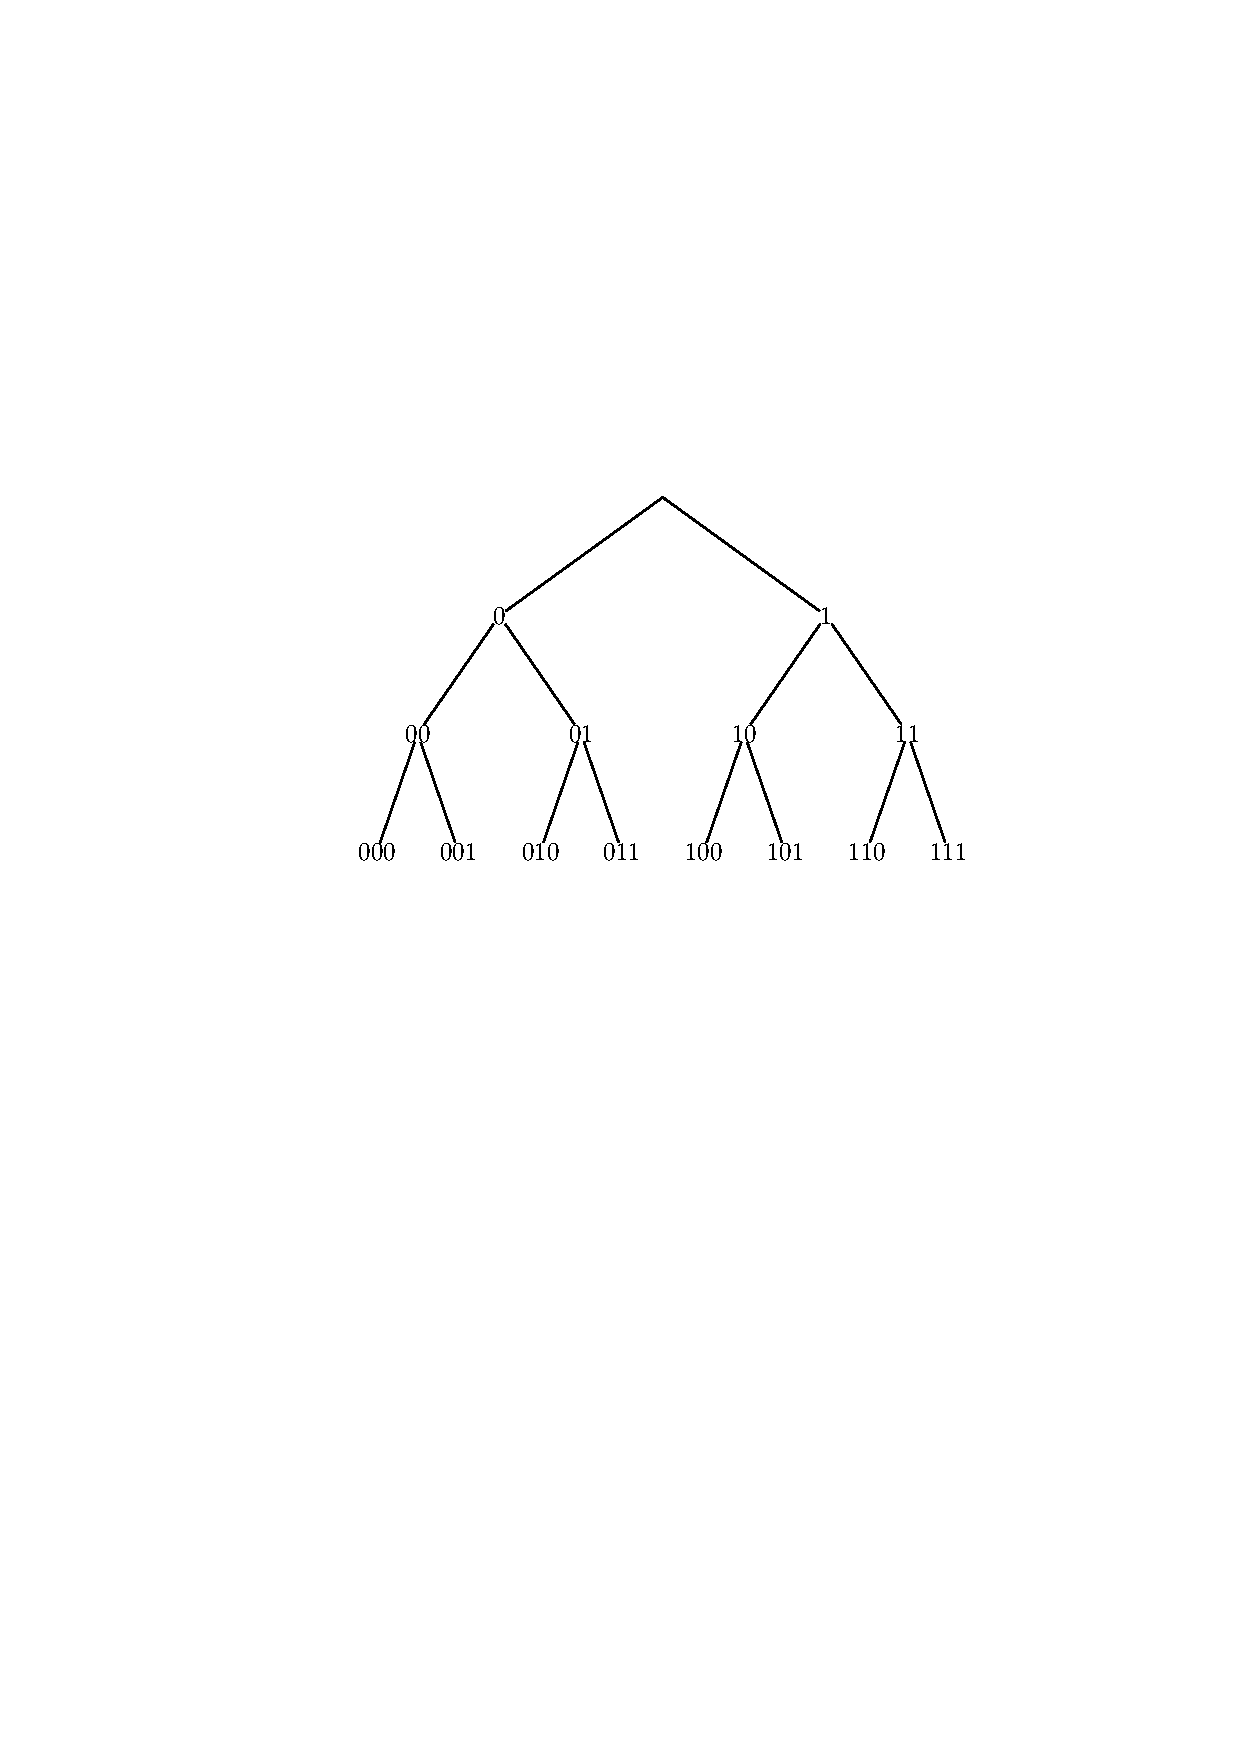
\includegraphics[scale=0.75]{arbol} 
\end{center}
\caption{Los nodos de un árbol binario correspondiente a $\mathbb{B}^{3}$}
\label{fig:RepresentacionArbol}
\end{figure}


\end{frame}

%%%%%%%%%%%%%%%%%%
\begin{frame}   \frametitle{Libre de prefijo utilizando árbol}   \small
 
 \begin{itemize}
\item Partimos de un código $C \subseteq \mathbb{B}^{*}$, y las palabras codificadas son los nodos del árbol binario. 

\item Las palabra codificada $q$ es un \textbf{prefijo} de otra palabra codificada $q'$ si el único camino de $q'$ a la raíz del árbol pasa a través de $q$.

\item  $C$ está \textbf{libre de prefijo}, para cada palabra codificada $q$, ninguno de los descendientes de $q$ puede ser una palabra codificada.

 \begin{itemize}
\item Por tanto podemos ignorar todos los nodos que son descendientes de $q$. 
\end{itemize}

\item Si ignoramos todos aquellos nodos que no son palabras codificadas ni prefijos de palabras codificadas, tendremos un árbol binario finito, y las palabras codificadas de C son sus hojas.
\end{itemize}
 

\end{frame}

%%%%%%%%%%%%%%%%%%
\begin{frame}      \small
 

\begin{ejemplo}

Representar el código  C = \{0, 10, 110, 111\} mediante un árbol.

\end{ejemplo}

\pause

\begin{figure}[!hbtp]
\begin{center}
	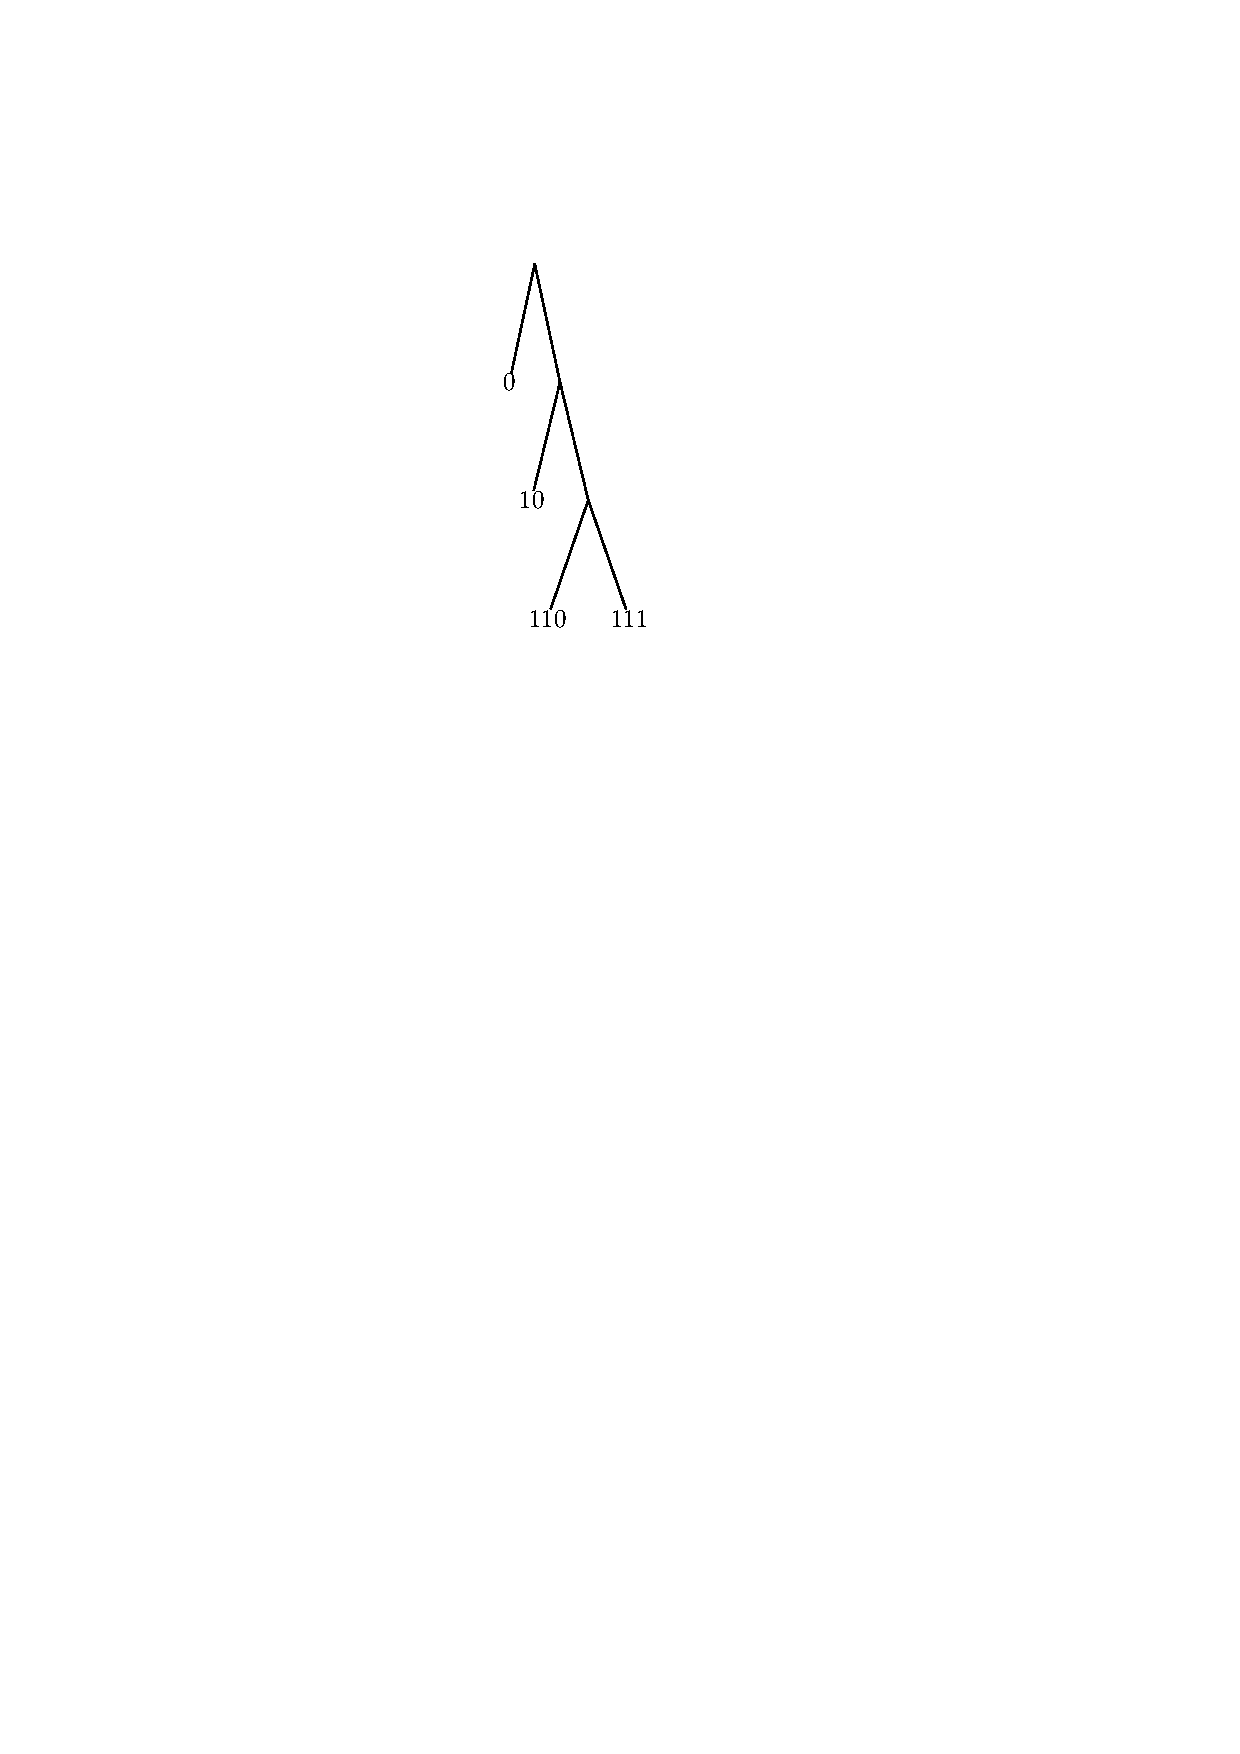
\includegraphics[scale=0.75]{ejArbol} 
\end{center}
%\caption{\small {Las palabras codificadas están representadas por las hojas en el árbol}}
\label{fig:ejeArbol}
\end{figure}

\end{frame}
%%%%%%%%%%%%%%%%%%


\begin{frame}      \small
 

 
 \begin{ejercicio}
Dibuja el árbol que representa el código PF $s_{1}  \mapsto 00$,  $s_{2}  \mapsto 010$,  $s_{3}  \mapsto 100$,  $s_{4}  \mapsto 111$ y etiqueta cada hoja con el símbolo correspondiente. ¿Es posible extender este código sin destruir la propiedad PF?
\end{ejercicio}


 \begin{ejercicio}
El alfabeto ternario T = \{0, 1, 2\}. Construya un árbol representando el código ternario con las palabras codificadas 02, 101, 120, 221, 222. ¿Es posible extender este código sin destruir la propiedad PF?
\end{ejercicio}

 \begin{ejercicio}
Tenemos el problema de representar los números 1, 2, 3, 4, 5, 6 mediante un  código binario PF, de tal forma que la longitud total de las palabras codificadas sea tan pequeña como sea posible. Construya un código que cumpla las condiciones, utilizando la representación de árbol como guía.

%$ 6 \mapsto 0$ entonces $ 5 \mapsto 10,  4 \mapsto 00$ y ya no hay más que hacer. Si no utilizamos palabras de longitud 2, entonces existe una solución $n_1=1, n_2=0, n_3=3, n_4=2$, con longitud total 18. Si no utilizamos las palabras de longitud 1, tenemos $n_1=0, n_2=2, n_3=4$ con longitud 16.

\end{ejercicio}

\end{frame}

%%%%%%%%%%%%%%%%%%

\section{El número Kraft-McMillan}

\begin{frame}    \frametitle{El número Kraft-McMillan}  \small

\begin{itemize}
\item Dado un código $c: S\rightarrow T^{*}$, sea $n_{i}$ el número de símbolos en S que son codificados por cadenas de longitud $i$ en $T^{*}$. 
	\begin{itemize}
		\item En otras palabras, $n_{i}$ es el número de $s \in S$ tal que $c(s)$ está en $T^{i}$.  
        \item Si tengo la codificación: 

        \begin{itemize}
            \item $a \mapsto 00$, $ b  \mapsto 010 $,   $ c  \mapsto 1001 $, $ d  \mapsto 1010 $, $ e  \mapsto 1100 $, $ f  \mapsto 1101 $, $ g  \mapsto 1111 $
              \item $n_2 = 1$, $n_3 = 1$, $n_4 = 5 $
        \end{itemize}
	\end{itemize}

\item Si M es la longitud máxima de una palabra codificada, nos referimos a los números $n_{1}, n_{2},\ldots,n_{M}$ como los \textbf{\underline{parámetros de c}}. 

\item En los diagramas de árbol, $n_{i}$ es el número de palabras codificadas en el nivel $i$.



\end{itemize}

\end{frame}
%%%%%%%%%%%%%%%%%%


\begin{frame}      \small

\begin{itemize}

\item Cuando $|T| = b$ el número de cadenas de longitud $i$ en $T^{*}$ es $|T^{i}| = b^{i}$. 

\item Por definición, un código $c: S\rightarrow T^{*}$ es una inyección, por lo que los parámetros deben satisfacer $n_{i} \leq b^{i}$. 

\item La fracción  $\frac{n_{i}}{b^{i}}$ representa la proporción de las palabras de longitud $i$ que son utilizadas como palabras codificadas.

\end{itemize}
 
 \begin{definicion} [Número Kraft-McMillan]\label{KMnumber}
El número Kraft-McMillan asociado con los parámetros $n_{1}, n_{2},\ldots,n_{M}$, y la base $b$ es definida como:
\begin{center}
$K=  \sum_{i=1}^{M} \frac{n_{i}}{b^{i}}    =  \frac{n_{1}}{b^{1}}   +  \frac{n_{2}}{b^{2}}   + \ldots + \frac{n_{M}}{b^{M}}  $
\end{center}


\end{definicion}

Por ejemplo si $n_{1}=1, n_{2}=2, n_{3}=1$ y b =2, entonces\\

\begin{center}
  K = 1/2 + 2/4 + 1/8 = 9/8.
\end{center}


\end{frame}

%%%%%%%%%%%%%%%%%%


\begin{frame}      \small
 
 Estableceremos dos importantes resultados sobre la existencia de códigos b-arios.

\begin{itemize}
\item Si $K \leq 1$ para un conjunto de parámetros $n_{1}, n_{2}, \ldots, n_{M}$ entonces existe un código PF b-ario con esos parámetros.
\item Los parámetros de un código UD b-ario deben satisfacer la condición $K \leq 1$.
\end{itemize}

Tomando estas dos consideraciones, tenemos que si tenemos un código UD con ciertos parámetros, entonces hay un código PF con los mismos parámetros.

\end{frame}


%%%%%%%%%%%%%%%%%%


\begin{frame}      \small
 
 \begin{ejemplo}
Construya un código binario con parámetros  $n_{2}=2, n_{3}=3, n_{4}=1$.
\end{ejemplo}

\pause
\textit{\underline{Solución}}:\\

 Primero verificamos que la condición $K \leq 1$ sea satisfecha:

\begin{center}
 K = 2/4 + 3/8 + 1/16 = 15/16.
\end{center}
 
 \begin{itemize}
\item  Para construir el código, ya que $n_{2}=2$, comenzamos con dos palabras codificadas de longitud 2, 00 y 01. 

\item  La condición PF significa que no podemos utilizar ninguna palabra de longitud 3 de la forma $00*$ o $01*$, pero nos quedan otras cuatro posibles palabras, de la forma $1**$. 


\item En realidad solo necesitamos tres de las cuatro, por lo que escogemos 100,101 y 110 por ejemplo. 

\item Para finalizar, necesitamos solamente una palabra de longitud 4, la cual puede ser o 1110 o 1111.

\end{itemize}
 
 
 
 
 


\end{frame}


%%%%%%%%%%%%%%%%%%


\begin{frame}      \small
 
 \begin{teorema}\label{theorem:CPF}
Si $K \leq 1$ para los parámetros $n_{1}, n_{2}, \ldots, n_{M}$ entonces existe un código PF b-ario con esos parámetros.
\end{teorema}


 \begin{ejercicio}

Construya códigos binarios PF con los siguientes parámetros:
\begin{itemize}
\item $n_2 =1,n_3 =4,n_4 =3;$
\item $n_1 =1,n_2 =0,n_3 =2,n_4 =3,n_5 =2.$
\end{itemize}

\end{ejercicio}
\pause
\textit{\underline{Solución}}:\\
Primer caso tendríamos: 00, 010, 011, 100, 101, 1100, 1101, 1110\\

Segundo caso tenemos: 0, 100, 101, 1100, 1101, 1110, 11110, 11111
\end{frame}

%%%%%%%%%%%%%%%%%%


\begin{frame}      \small
 
 \begin{ejercicio}

Basándonos en el teorema \ref{theorem:CPF}, que podemos decir sobre la existencia de códigos ternarios PF (b=3) con los siguientes parámetros:

\begin{itemize}
\item $n_1 =0,n_2 =1,n_3 =12;$
\item $n_1 =0,n_2 =1,n_3 =12,n_4 =40$
\end{itemize}

\end{ejercicio}
\pause

\textit{\underline{Solución}}:\\

Primer caso: $\frac{0}{3} + \frac{1}{3^2}+ \frac{12}{3^3}$ = $\frac{15}{27}\leqslant 1$\\

Segundo caso: $\frac{0}{3} + \frac{1}{3^2}+ \frac{12}{3^3}+ \frac{40}{3^4}$ = $\frac{85}{81} > 1$


\pause
 \begin{ejercicio}

Si la conclusión del anterior ejercicio es que debe existir un código PF, construya uno.

\end{ejercicio}

\end{frame}

%%%%%%%%%%%%%%%%%%

\subsection{UD implica $K \leq 1$}
\begin{frame}    \frametitle{UD implica $K \leq 1$}     \small
 
\begin{itemize}
\item Los parámetros de un código UD  $(n_k)$ deben satisfacer $K \leq 1$.  

\item Sea $c: S\rightarrow T^{*}$ un código con parámetros $n_{1}, n_{2}, \ldots, n_{M}$. 

\item M es la longitud de la palabra codificada más larga para \textbf{un único símbolo}, la \textbf{máxima longitud del código para una cadena de $r$ símbolos es $rM$}.

 
\end{itemize}

\begin{definicion} [$q_{r}(i)$]\label{qr}
Dado $r \geq 1$, sea $q_{r}(i)$ el número de cadenas de longitud r que son codificadas por cadenas de longitud i $(1\leq i \leq rM)$. 

En particular $q_{1}(i)=n_{i}$. 
\end{definicion} 
 Mostraremos a continuación que los parámetros $n_{i}$ determinan el número de $q_{r}(i)$, para todos los r.

\end{frame}

%%%%%%%%%%%%%%%%%%


\begin{frame}      \small
 
 \begin{ejemplo}

Supongamos que $c: S\rightarrow T^{*}$  es un código con parámetros $n_{1}=2$, $n_{2}=3$. ¿Cuales son los valores para $q_{2}(i)$?
\end{ejemplo}
 
\pause
\textit{\underline{Solución}}:\\

\begin{itemize}
\item  Sea \textbf{$xy$ una cadena de longitud 2} en S. Ya que c(x) y c(y) tienen o longitud 1 o 2, c(xy) tendrá una longitud 2,3, o 4.


\begin{itemize}
\item Si c(xy) tiene \textbf{longitud 2}: c(x) y c(y) deben tener ambos longitud 1. Ya que $n_{1}=2$, hay $2\times 2$ cadenas posibles xy. Por tanto $q_{2}(2)=4$

\item Si c(xy) tiene \textbf{longitud 3}: c(x) debería  tener longitud 1 o 2, y  c(y) debería tener longitud 2 o 1, respectivamente. Debido a que $n_{1}=2$ y $n_{2}=3$, hay $2\times 3$ + $3 \times 2$ posibles cadenas xy. Por tanto  $q_{2}(3)=6+6=12$

\item Si c(xy) tiene \textbf{longitud 4}: c(x) y c(y) deben tener ambos longitud 2. Ya que $n_{2}=3$, existe $3	\times 3$ posibles cadenas xy. Por tanto $q_{2}(4)=9$.
\end{itemize}
\end{itemize}





\end{frame}

%%%%%%%%%%%%%%%%%%


\begin{frame}      \small

Definiremos la función de generación para la secuencia  $q_{r}(1)$,$q_{r}(2)$,$\ldots$ $q_{r}(M)$ como sigue:

\begin{center}
$Q_{r}(x)=q_{r}(1)x+q_{r}(2)x^{2} +\ldots +q_{r}(rM)x^{rM}.$
\end{center}
 
 
\begin{lema}
Para todos $r\geq 1$, $Q_r(x)=Q_1(x)^r$
\end{lema}

\begin{teorema}\label{UDK1}
Si existe un código b-ario univocamente decodificable, con una serie de parámetros, entonces su Kfraft-McMillan número satisface que  $K \leq 1$
\end{teorema}


\end{frame}

%%%%%%%%%%%%%%%%%%


\begin{frame}      \small



Teorema \ref{UDK1} puede ser combinado con el teorema \ref{theorem:CPF} de la siguiente forma:

\begin{center}
código UD existe $\Longrightarrow K\leqslant 1 \Longrightarrow$ código PF existe
\end{center}

la existencia un código UD con unos parámetros dados implica la existencia de un código PD con los mismos parámetros. \\
\vspace{15pt}
Existe un código UD con ciertos parámetros sii existe un código PF con los mismos parámetros y esto sucede sii $K\leqslant 1$.
\end{frame}

%%%%%%%%%%%%%%%%%%


\begin{frame}      \small
 
 
  \begin{ejercicio}

 Supongamos que queremos construir un código UD para 12 símbolos utilizando palabras binarias que no excedan de longitud 4. Establezca una lista de todos los conjuntos de parámetros $n_1,n_2,n_3, n_4$ para el cual existe un código apropiado.
 \end{ejercicio}
 
  \pause
  \textit{\underline{Solución}}:\\
  
  Los parámetros $n_1,n_2,n_3, n_4$ deben satisfacer:
  
\begin{center}
  $n_1+n_2+n_3+n_4=12$ 
\end{center}
\begin{center}  
  $n_1/2+n_2/4+n_3/8+n_4/16\leqslant 1$ 
\end{center}

  Multiplico por 16: $8 n_1 + 4 n_2 + 2 n_3 + n_4 \leqslant 16$ , despejo $n_4$, $n_4 =12-n_1- n_2-n_3$  y sustituyo $n_4$ tengo que $7 n_1 + 3 n_2 + n_3 \leqslant 4$.\\ 
  Por tanto $n_1=0$ y $n_2 \leqslant 1$. \\
  Ahora podemos establecer una lista de posibilidades:
  
  
  \begin{center}
  \begin{tabular}{cccccccc}
$n_2:$ & 1   &  1 & 0 & 0  & 0 &0 &0\\
$n_3:$ & 1   &  0 & 4 & 3  & 2 &1 &0\\
$n_4:$ & 10 & 11& 8 & 9  & 10 & 11 &12\\

\end{tabular}
\end{center}



\end{frame}

%%%%%%%%%%%%%%%%%%


\begin{frame}      \small
 
 
   \begin{ejercicio}

Sea $S = \{s_1,s_2,\ldots ,s_6\}$ y T = \{a,b,c\}, y tenemos un código definido por 
$s_1\mapsto a$, $s_2\mapsto ba$, $s_3\mapsto  bb$,$s_4 \mapsto bc$, $s_5 \mapsto  ca$,$s_6 \mapsto cb$.

Establezca la función generadora $Q_1(x)$ y $Q_2(x)$  

 \end{ejercicio}
 
 \pause  
 \vspace{1cm}
  \textit{\underline{Solución}}:\\
   \vspace{0.5cm}
Tenemos $n_1=1, n_2=5$, por lo que $Q_1(x) = x + 5x^2$ y \\por el lema 1 ( $r\geq 1$, $Q_r(x)=Q_1(x)^r$) $\rightarrow$
$Q_2(x) = Q_1(x)^2$ $\rightarrow$ 

$Q_2(x) = (x + 5x^2)^2 \rightarrow$ 

$Q_2(x) = x^2 + 10x^3 + 25 x^4$

 
\end{frame}


%%%%%%%%%%%%%%%%%%


\begin{frame}      \small
 

 \begin{ejercicio}

En el ejercicio anterior, ¿Qué significa el coeficiente $x^4$ en $Q_2(x)$?
 \end{ejercicio}
 
  \pause
  \textit{\underline{Solución}}:\\
  
   El coeficiente $x^4$ en $Q_2(x)$ es el número de palabras S de longitud 2 que son representadas por palabras T de longitud 4. Esas 25 palabras son todas las palabras $s_is_j$ con i,j $\in \{2,3,4,5,6\}.$
\end{frame}
%%%%%%%%%%%%%%%%%%


%%%%%%%%%%%%%%%%%%


\begin{frame}      \small
 
 \begin{ejercicio}

Sea $S = \{a, b, c, d, e, f, g\}$ y tenemos un código binario definido como 
$a\mapsto 00$, $b\mapsto 010$, $c\mapsto  011$,$d \mapsto 1000$, $e \mapsto  1001$,$f \mapsto 1101$,$g \mapsto 1111$.

Establezca la función generadora $Q_1(x)$ y $Q_2(x)$  

 \end{ejercicio}
 
 \pause
 \textit{\underline{Solución}}:\\

Tenemos $n_2=1, n_3=2, n_4=4$, por lo que $Q_1(x) = x^2 + 2x^3+ 4 x^4$ y por ende $Q_2(x) = x^4 + 4x^5 + 12 x^6 + 16 x^7+ 16 x^8$

\end{frame}

%%%%%%%%%%%%%%%%%%

\subsection{Principio de Conteo}
\begin{frame}   \frametitle{Principio de Conteo}   \small
 
 
 \begin{teorema}[Principio de Conteo]

Sea $c: S\rightarrow T^{*}$ un código que para todo $s\in S$, la longitud c(s) no es mayor que M. Dado $r \geq 1$, sea $q_r(i)$ el número de cadenas de longitud r en S que son codificados por cadenas de longitud i en T ($1\leq i \leq rM$). Sea $Q_r(x)$ la función de generación
 
\begin{center}
$Q_{r}(x)=q_{r}(1)x+q_{r}(2)x^{2} +\ldots +q_{r}(rM)x^{rM}.$
\end{center} 
 
Entonces $Q_{r}(x)=Q_{1}(x)^r$.

\end{teorema}
 

\end{frame}




\begin{frame} %\frametitle{Preguntas}

%\begin{center}
%¡Gracias por su atención!\\
%\end{center}
\vspace*{2cm}

\begin{center}
\textbf{José A. Montenegro Montes} \\

\textit{Dpto. Lenguajes y Ciencias de la Computación}\\
\textit{ETSI  Informática. Universidad de Málaga}\\
\textbf{jmmontes@uma.es}\\
%\href{https://twitter.com//monteDocencia}{
%
\includegraphics[height=0.05\textheight]{twitter.jpg}}
\end{center}

\vspace*{1,5cm}


\includegraphics[height=0.15\textheight]{logoUma.jpg} \hspace*{3.6cm}

\includegraphics[height=0.15\textheight]{logoInf.jpg}   \hspace*{3.7cm}

\includegraphics[height=0.15\textheight]{logoLcc.jpg}  



\end{frame} 

\end{document} 